\documentclass[handout]{beamer}

\usepackage[utf8]{inputenc}
\usepackage[frenchb]{babel}
\usepackage{amsmath}
\usepackage{graphicx}
\usepackage{tikz}

\title{Semaine du Numérique}
\author[G. Guisez, J. Hennani, V. Hiairrassary, W. Tassoux]{Grégoire Guisez, Jamal Hennani, Victor Hiairrassary, William Tassoux}
\institute{Polytech' Montpellier, Université Montpellier 2}
\date{14 mai 2012}


\usetheme{Warsaw}

\AtBeginSection[]{
   \begin{frame}
   \begin{center}{\Large Plan }\end{center}
       \tableofcontents[currentsection,hideothersubsections]
   \end{frame} 
}


\begin{document}

\small 

%\logo{
\includegraphics[scale=0.2]{images/logoPolytech.jpg}}
%\setbeamertemplate{sidebar left}
%{
%    \logo{
\includegraphics[scale=0.05]{images/logoUm2.jpg}}
%    \vfill
%    \rlap{\hskip0.1cm\insertlogo}
%    \vskip8pt
%}


\begin{frame}
    \titlepage

    
\includegraphics[scale=0.2]{images/logoPolytech.jpg}
    \hfill
    \hskip8pt
    
\includegraphics[scale=0.05]{images/logoUm2.jpg}
\end{frame}


\begin{frame}{Introduction}
    \begin{block}{Introduction}
 		 Ce projet vise à mettre en place une partie de la semaine du numérique qui se déroulera lors des années à venir.

		 On peut le décomposer en 2 sous projets:
		\begin{itemize}
			\item Lecteur de carte
			\item Site web
		\end{itemize}
	\end{block}

	\begin{block}{Semaine du Numérique}
	    La semaine du numérique correspond à un évenement ponctuel coordonnée 
    par Polytech, en collaboration avec des intervenants extérieurs. Cette 
    dernière sera sanctionnée comme tout autre unité d'enseignement par un QCM.
	\end{block}	
\end{frame}


\begin{frame}{Plan}
 	\tableofcontents
\end{frame}

\chapter{Site web}
    \section{Cahier des charges}
    \section{Modélisation}
    \section{Framework}
        \cite{ref_framework_mvc}

    \section{Check list}
    \section{Recommandations}


\chapter{PDFBox}
    Le site web comprend une partie permettant aux éleves de consulter des cours 
en ligne, par les conférenciers soit en récupérant des pdf ou alors en visionnant
des "diapositives". Ces dernières correspondent à des pages de fichiers pdf qui
ont été au préalable convertit en image. 

    Cela a été possible en utilisant un projet open source PDFBox \cite{pdfbox}.
\newline
\newline

    \begin{figure}[h]
        \begin{center}
            
\includegraphics[scale=0.6]{PDFBox.png} 
        \end{center}

        \caption{Logo PDFBox}
        \label{Logo PDFBox}
    \end{figure}

\newpage



	\section{Présentation du projet PDFBox}
	PDFBox est une librairie open source codée en java, permettant de manipuler 
des documents pdf. Elle permet la création de manipuler les fichiers PDF de 
nombreuses façon.

	PDFBox est sous license Apache License v2.0, ce qui en fait un lobiciel libre 
et open source.

	Principales fonctionnalités:
	\begin{itemize}
		%expliquer pk difficile de differencier paragraphe si vraiment necessaire au rapport
		\item Extraction de texte.
		      Cette fonction est toujours au stade de devloppement car il est difficile de 
              différencier deux paragraphes différents dans un fichier pdf (la position 
              du texte est donnée par des positions absolue, ce qui permet de disposer 
              le texte exactement la où on le souhaite).  
		\item Fusion de documents PDF. 
		\item Encrypter/Décrypter.
		\item Créer un PDF depuis un fichier texte.
		\item Création d'images à partir d'un document PDF. C'est ce qui va 
              principalement nous intérésser. C'est cette dernière qui servira à 
              fournir les diapositives que les élèves pourront consulter à partir 
              du site web.
		\item Imprimer un PDF.
	\end{itemize}

		Il faut savoir que la fonction convertissant un pdf en images est encore
    au stade de développement. Ce qui veut dire que  les fonctionnalités ne sont 
    pas encore toutes implémentées ou encore que certains bugs subsistent encore.

        Ci-dessous nous allons expliquer les problèmes que nous avons rencontrés,
    ainsi que la manière dont nous avons résolus chacun d'entre-eux.

        Avant toute chose, il est important de noter que la résolution à ceux-ci
    à été possible grâce à la documentation de PDFBox et à celle de la classe 
    java.awt.Font ainsi qu'au débugueur inclus dans l'environnement de dévelopement 
    Eclipse.


	\section{MediaBox et CropBox}
        Lors de nos tests, nous nous sommes rendues compte qu'il pouvait y 
    avoir un problème de conversion avec un fichier pdf contenant à la fois une 
    "cropbox" et une "mediabox". Il faut savoir que lors de la visualisation d'un 
    document pdf, par défaut, on ne voit que la partie que l'auteur veut que l'on 
    voit. Ce procédé est par exemple utilisé dans les imprimeries. 

		\begin{itemize}
			\item La cropbox correspond  à la partie visible par tous du document, 
                  c'est celle qui est destinée à être vue.
			\item La mediabox comprend la cropbox et correspond à la totalité 
                  réelle du document et non pas seulement à la partie visible 
                  lors de la lecture du fichier avec Adobe Reader par exemple. 
		\end{itemize}

        %TODO: Image contenant cropbox et mediabox 
    
     \begin{figure}[h]
            \begin{center}
            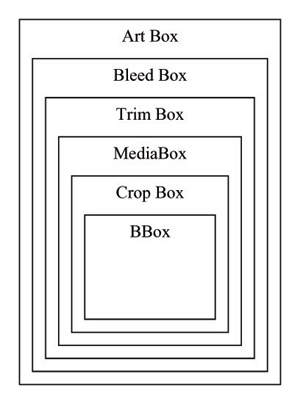
\includegraphics[scale=0.6]{crop_media_box.jpg} 
            \end{center}
            \caption{hiérarchie des différentes "box"}
            \label{hiérarchie des différentes "box" }
     \end{figure}

	        Ce premier problème se rapporte au fait de ne pas pouvoir convertir
        une page en entier si une cropbox était spécifiée (la médiabox l'est 
        obligatoirement elle). Pour cela, il a fallut envoyer les bonnes dimensions 
        de pages à chaque fois qu'une image est crée, et cela sans utiliser la fonction
        getcropbox retournant un objet de type PDRectangle et qui ne fonctionne 
        pas correctement (lance un null pointeur exception). On a donc changé le
        code pour faire appel à la fonction findcropbox() qui elle fonctionne 
        correctement.


	%TODO: Dire quel fichier et quelles lignes on été modifiés


    \lstset{language=Java}
	\begin{lstlisting} 
private static void changeCropBoxes(PDDocument document,float a, float b, float c,float d)
{
	List <PDPage> pages = document.getDocumentCatalog().getAllPages();
	for( int i = 0; i < pages.size(); i++ )
	{
        System.out.println("resizing page");
        PDPage page = (PDPage)pages.get( i );
        PDRectangle rectangle = new PDRectangle();
        rectangle = page.getMediaBox();
        a=0;
        rectangle.setLowerLeftY(a);
        rectangle.setLowerLeftY(b);
        rectangle.setUpperRightX(c);
        rectangle.setUpperRightY(d);

        page.setMediaBox(rectangle);
        page.setCropBox(rectangle);
	 }
}
 \end{lstlisting}

        Une fois que les dimensions recherchées sont récuperées, on les affectes
    aux pages du document PDF l'on veut convertir. Ainsi on obtient bien les bonnes 
    dimensions de pages.



    \section{Polices embarquées}
        Il faut savoir que suivant les softwares employés pour créer les PDF et
    les polices utilisées, il est possible de ces dernières soient directement
    inclues dans le fichier final. Cela est autorisé par la norme ISO régissant 
    ce type de fichier. Or en n interne, la gestion des polices est faites via 
    classe "java.awt.Font". Et malheuresement, cette dernière nécessite de travailler
    avec des polices complètes.

        Il arrive donc que suivant les fichiers à transformer en images, si la police 
    est contenue dedans, le resultats soit illisible, dû à la confusion par rapport
    au caractère manquant.

        %TODO: Image de diapositive erronée.

        Comme mentionnée précédemment, certains fichiers PDF, peuvent contenir eux 
    même la définition ainsi que les glyphes correspondants aux caractères utilisées dans 
    le document. Cependant, si ces dernières ne sont pas complètes, il subsistait
    quelques erreurs.

        Nous avons essayer de modifier nous même les polices incriminées mais 
    sans résultats probants. Nous avons donc patché le code une deuxième fois 
    en donnant la police système si le document en utilisait une interne.

        De ce fait tous les documents se verront ecris avec cette police mais 
    on garde l'avantage de garder partiellement le style d'écriture 
    (soulignement, couleur, taille).




%TODO: Donner les diffs en annexe




\chapter{Lecteur de cartes}

Afin de vérifier l'assiduité des élèves lors des conférences, nous mettons en
place un système de badge.

Il nous fallait une solution alliant plusieurs critères comme un coût limité,un temps
de développement réduit et de la fabilité.

    \section{Historique}

Dès le début du projet, Monsieur Berry nous a proposé plusieurs pistes à 
explorer pour le badge en lui même. Il fallait que chaque participant aux
conférences puisse être identifié de manière unique:

\begin{itemize}
\item Money Kart: C'est une entreprise basée près de Grenoble, spécialisée
dans la création de cartes à puce, notamment Moneo. L'avantage de cette solution
résidait dans la design des cartes. On aurait pu les faire graver
de façon à faire un buzz autour de la Semaine du Numérique. De plus la société
vendait également des lecteurs prêts à l'emploi.
Malheuresement, il nous fût impossible d'obtenir un devis de la part d'un
commercial, même après de multiples relance. Cette solution nécéssitait aussi
un investissement financier.

\item Carte étudiant: Rapidement cette solution à fait l'unanimité. En effet,
elle était bien plus facile à mettre en place: chaque titulaire de carte délivrée
par l'UM2 possède un numéro unique, appelé numéro Mifare, accessible grâce à
la technologie RFID. Or Polytech possède une base de données faisant le lien entre
ce numéro et les élèves.
\end{itemize}

    \section{RFID et Mifare}

RFID, de l'anglais ``radio frequency identification'' est une techonlogie 
mise au point pour permettre de lire à distance des données contenues dans des
marqueurs, les étiquettes RFID.

    \begin{figure}[h]
        \begin{center}
            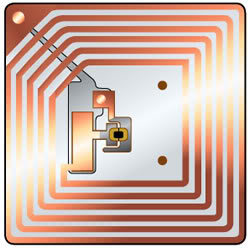
\includegraphics[scale=0.6]{images/RFIDtag.jpg} 
        \end{center}

        \caption{Etiquette RFID}
        \label{Etiquette RFID}
    \end{figure}


C'est une technologie employée quotidiennement par tout le monde puisqu'elle
est utilisée dans les cas suivants:

    \begin{itemize}
    \item Passeport bimométrique français
    \item Accès transport public, comme le tramway de Montpellier
    \item Inventaires
    \end{itemize}

Mifare est une des technologies de carte à puce sans contact les plus répandues
dans le monde avec 3,5 milliards de cartes et 40 millions de modules de lecture/encodage.

Ces deux technologies respectent les normes ISO.

\section{MFR120U}

Rapidement après le début du projet, Mr Berry nous à mis en contact avec Mr
Cathebras, directeur du département ERII à Polytech'. En effet, il souhaitait lui
aussi mettre en place un système de présence informatisé, pour éviter de devoir
le faire sur papier, avant de le reporter sur l'ordinateur.

Or il avait déjà creusé de son côté, puisqu'il avait acheté un lecteur de carte 
Mifare, appelé module MFR120U, pour la somme de 120\euro. Ce lecteur présentait néanmoins
plusieurs inconvénients majeurs:

    \begin{itemize}
        \item Programme d'utilisation exclusivemment sous les plateformes Windows.
        \item Liaison série-USB avec l'ordinateur par câble, ce qui nécessitait 
              à l'utilisateur d'installer un driver fournis également que pour
              Windows.
        \item Difficulté à savoir si la lecture de la carte avait réussi ou non.
    \end{itemize}

Par contre il posséde un écran LCD, ce qui peut se révéler assez pratique pendant

Mr Cathebras avait donc demandé à un de ses collègues de travail du département
ERII, Mr Tamby, s'il pouvait concevoir un module qui répondrait plus à ses attentes.
De notre côté, nous devions nous occuper de toute la partie software.

C'est ici que nous intervenont. Début février 2012 nous avons recontré Mr Cathebras,
et nous avons pu discuter de l'intérêt commun à développer un tel lecteur. En effet,
s'il venait à faire ses preuves en plus lors des conférences, il pourrait se voir
industrialisé afin de voir son utilisation généralisée à Polytech. Il nous à donc
confié le MFR120U pour que nous puissions nous faire la main dessus.

    \begin{figure}[h]
        \begin{center}
            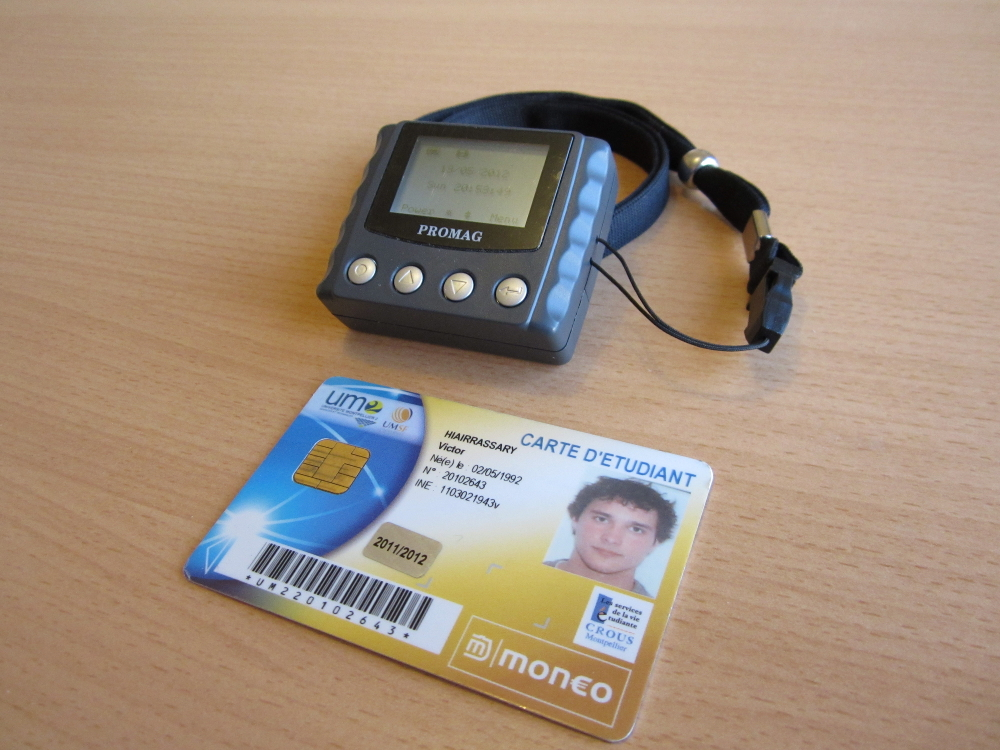
\includegraphics[scale=0.75]{images/mfr.jpg}
        \end{center}
        \caption{MFR120U}
        \label{MFR120U}
     \end{figure}  

De plus il nous a fourni la documentation du lecteur. Or celle-ci nous fût d'un
grand secours par la suite puisqu'elle comprenait tout le protocole de communication
utilisé par le lecteur, ainsi que de nombreuses autres caractéristiques.

    \begin{itemize}
    \item Fabricant de la puce: Prolific Technology Inc. Les drivers pour Windows
          et MacOS X sont disponibles sur leur site web \cite{prolific}
    \item Baud rate: 19200
    \item Communication série 8N1 : 8 bits de donnés, aucun de parité, et 1 de stop
    \item Possibilité de lire les cartes Mifare, ainsi que d'autres normes
    \item En interne, le lecteur possède une mémoire capable de stocker 8000
          lectures de badge (date, heure, et informations contenues sur la carte)
    \end{itemize}

En interne, la gestion des enregistrements fonctionne grâce à un curseur.
De base, il pointe sur le premier enregistrement. On ne peut que demander le suivant,
ce qui à pour effet d'incrémenter ce curseur et de renvoyer la nouvelle valeur
pointée, ou faire un ``rollback'', c'est à dire remettre le curseur sur le tout
premier enregistrement.

Le lecteur possédait également un système de droit d'accès avec un mot de passe.

Le programme que nous devions développer était en somme assez simple, puisqu'il
devait offrir une interface permettant de se connecter au lecteur, de récupérer les
données contenues suivant certains critères, les supprimer en mémoire si nécéssaire,
et enfin les envoyer sur une base de données distante.

La version fonctionnelle pour le MFR120U (sans l'envoi en base de données)
est disponible dans le repository git sous le tag v0.9-mfr120u.

        \section{Caractère multi-plateformes}

Afin de répondre à la demande multi-plateforme des professeurs, nous nous 
sommes naturellement tourné vers le language C++. En effet, celui-ci offre un accès
proche de la machine, intéréssant pour la communication série notamment. De plus,
un étudiant ERII 3, Arthur Hiairrassary, à mis à notre disposition la bibliothèque
pour faire transiter des informations séries.

Par contre, nous avons développé avec le nouveau standard C++11. Ainsi
dans le code nous trouvons l'utilisation des concepts suivants:

    \begin{itemize}
    \item Variadics templates
    \item Fonctions lambdas
    \item Rvalues references
    \item Move-constructor
    \end{itemize}

L'inconvénient de cela est bien sur le support par les compilateurs de cette
norme. Par exemple, msvc, le compilateur de Microsoft, ne prend en charge que peu
de ces fonctionnalités, et n'est donc pas à même de compiler le code, même avec la
beta de Visual Studio 2011.

Néanmoins, l'utilisation de ce standard nous à permis de s'affranchir de nombreuses
restrictions, et par conséquent un développement plus rapide, mais surtout bien
plus sûr. En effet la S(T)L est bien plus avancée.

De plus, l'inconvénient dû au compilateur msvc fût de courte durée puisqu'il
existe g++ et clang++, qui eux supportent en grande partie le nouveau standard.
Et en plus ils sont multi-plateformes! Le programme a pour l'instant été testé 
avec succès dans les conditions suivantes:

    \begin{itemize}
    \item Windows 7, 64 bits, MinGW 4.6.1
    \item MacOS X 10.7, 64 bits, clang++ 3.0 (sous machine virtuelle)
    \item Linux >= 3.1, 64 bits, g++-4.6
    \end{itemize}

Afin de permettre une compilation aisée sur toutes ces plateformes, nous avons
optés pour l'utilisation de CMake afin de générer l'ensemble de l'environnement de
façon automatique.

    \section{Prototype}

Début décembre, nous avons pu rencontrer Mr Tamby, en charge de développer le
prototype du nouveau lecteur. Durant notre première réunion, il nous a donné
bon nombre de renseignements et conseils. De notre côté, nous lui avons fourni
l'ensemble des commandes que nous souhaitions retrouver dans le prototype final.

Aux alentours de mi-avril, il nous invite donc à voir le premier prototype.

    \begin{figure}[h]
        \begin{center}
            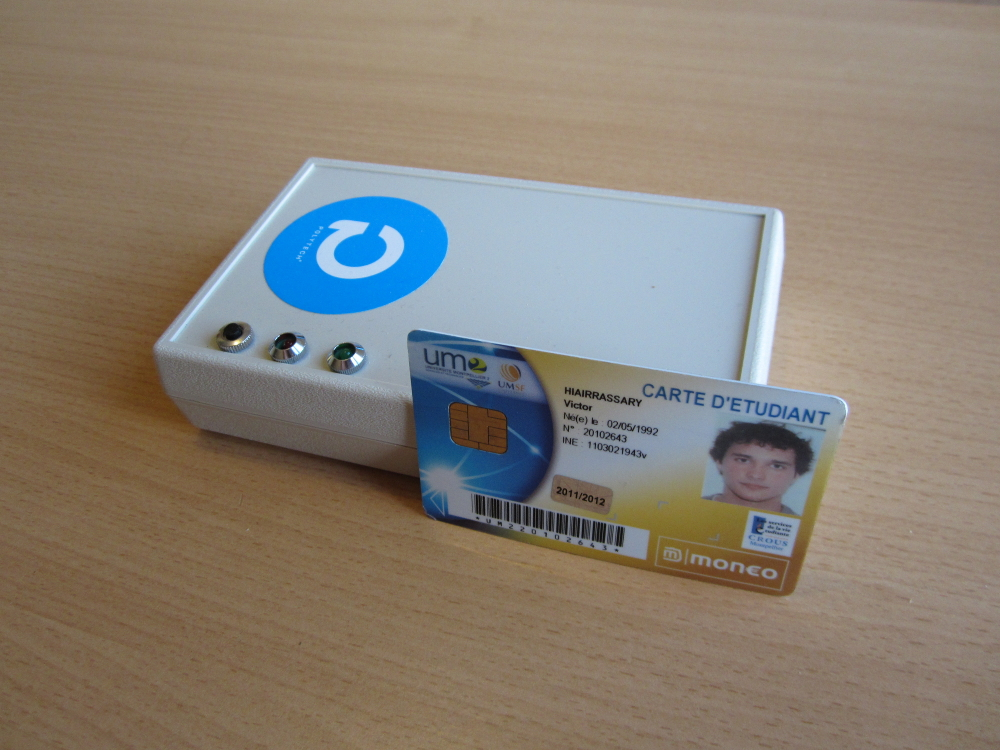
\includegraphics[scale=0.75]{images/proto.jpg} 
        \end{center}
        \caption{Prototype du lecteur}
        \label{Prototype du lecteur}
     \end{figure} 

Nous sommes alors très surpris par le respect dont Mr Tamby a fait preuve
durant la réalisation du module, tant au niveau électronique que firmware.
En effet il n'aura fallu changer que le baud rate, ainsi que quelques lignes
pour que le programme soit opérationnel pour ce lecteur !

De plus, plus besoin de câble, puisque le prototype fonctionne par Bluetooth,
conformément aux recommandations de Mr Cathebras. Cela engendrera aussi la disparition
du système de droit d'accès puisque pour pouvoir se connecter à un module Bluetooth,
il est possible de spécifier un code PIN.

Le firmware du lecteur est un mélange des langages C et assembleur, pour un total
d'environ 1700 lignes de code. Ci-dessous des brides du code, afin de montrer
que celui-ci reste très proche de la machine.

    \lstset{language=C}
    \begin{lstlisting} 
// Choix du sens des ports I/O
    // Registre OPTION_REG relatif aux interruptions
    OPTION_REG = 0b10000000;

    // Registre INTCON relatif aux interruptions
    INTCON = 0b11000000;
    ANSELH=0;

    // Detecter l'interruption sur RB4
    IOCB =0b00010000;
    \end{lstlisting}


    \lstset{language=[x86masm]Assembler}
    \begin{lstlisting} 
#asm

inter_suite:
	movwf	saveW		// sauvegarde du registre W	
	movf	STATUS,0
	movwf	savesta		// sauvegarde du registre STATUS
	movf    PCLATH,0
	movwf	savePCLATH

	bcf		PCLATH,4
	bcf		PCLATH,3

	bcf	    STATUS,RP0

// ...
    \end{lstlisting}

    \section{Protocole de communication}

Le protocole de communication utilisé n'est pas difficile. Il est orienté 
texte, puisqu'il repose sur le jeu de caractères ASCII, soit 8 bits pour chacun des
caractères, ce qui correspond sur les processeurs Intel en C++ au type char. 
Toute commande s'effectue de la sorte:

STX Command [Data] CR

Les caractères STX et CR, sont non-imprimables, prenant respectivement les
valeurs 0x02 et 0x0D. ``Commande'' est codée sur un seul caractère, alors que ``Data''
est optionnel et dépend de la commande. Pour le programme du prototype nous avons
entre autres:

    \begin{itemize}
    \item N: Retourne le nombre d'enregistrements
    \item E: Efface la mémoire des enregistrements
    \item T: Retourne la date du lecteur
    \end{itemize}

En retour à chacune des commandes, le lecteur renvoie une séquence, de la forme:

STX ReturnValue [Data] CR

En général, ``ReturnValue'' est le caractère A, 0x41, pour dire que
la commande s'est bien déroulé. ``Data'' est une nouvelle fois optionnel.

La liste exhaustive des commandes du protocole pour le prototype est disponible
en annexe du rapport. 

Attention, elles diffèrent quelque peu de celles du MFR120U, présentes sur 
la documentation officielle.

    \section{Architecture}

Le programme ``badger'' est décomposé en plusieurs dossier. 

Dans le dossier serial/ on trouve toute la bibliothèque concernant la communication
série. Elle utilise l'idiome de programmation Pimpl (Private Implementation), afin 
de séparer interface et implémentation. Cela est dû au fait qu'elle est implémentée
pour les systèmes POSIX d'un côté (Linux et MacOS), et Win32 de l'autre. Ces derniers
ne supportent pas de façon optimale la norme POSIX.

Le répertoire console/ contient quant à lui tout le système d'interpréteur.
Il est issu d'un projet de moteur de rendus 3D d'un des membres du projet.

Enfin le dossier badger/ contient le programme final, faisant appel à ceux
ci-dessus. Il contient de plus une classe permettant d'envoyer des requêtes SQL
à une base de données MySQL distante. Le programme fonctionne sous la forme d'un 
interpréteur de commandes.

    \section{Utilisation}

Ci-dessous, voici l'exemple d'utilisation sous Linux, une fois placé dans le
répertoire du binaire du programme badger:

    \begin{lstlisting}
./badger

open /dev/rfcomm0
count
send passwd 25-12-2011 10:00:00 17:00:00
erase
close
exit
    \end{lstlisting}

L'exemple ci-dessus, ouvre une connexion série sur le descripteur de fichier
/dev/rfcomm0. La commande ``count'' renvoie le nombre d'enregistrement contenus sur 
le module, alors que ``send'' envoie automatiquement dans une base de données (nommée
dans le code) tout les enregistrements effectués le 25-12-2011 entre 10H et 17H.
Enuiste ``erase'' vide la mémoire, ``exit'' ferme la connexion s'il elle existe, et
quitte le programme.

L'ensemble des commandes pour l'interpréteur est aussi disponible en annexe.

    \section{Recommandations et limites}

Actuellement, le plus gros manque dans ce programme (sans considérer une IHM) est
le manque de détection automatique du lecteur: en paramètre de la commande ``open''
l'utilisateur doit spécifier le descripteur de fichier, qui change d'une plateforme
à l'autre, voire de la version de l'OS employé ou du nombre de périphériques connectés:

    \begin{itemize}
    \item Windows: COMx, où x >= 1.
    \item MacOS X: /dev/tty.Polytech-ERII
    \item Linux: /dev/rfcommx, où x >= 0.
    \end{itemize}

Donc nous sommes encore dans la recherche d'une solution ``viable''. Par
rétro-ingéniérie grâce à un programme écoutant les ports séries; nous avons
trouvé comment le programme officiel reconnaissait si le lecteur MFR120U était 
connecté ou pas: au lancement le programme envoie sur tous les ports la commande
STX F CR, qui si elle est envoyé sur le MFR120U, retourne un résultat attendu.

Or cette façon nous dérange, dans le sens où l'on ne sait pas sur quel périphérique
nous allons envoyer cette commande, et encore moins qu'elle va être sa réaction...

\chapter{Environnement}
    \section{Règles de codage}
    Ci-dessous, voici les règles de codage utilisées tout au long du projet
ainsi que dans le rapport. Elles sont là pour permettre une cohérence tout au
long du développement, mais aussi et surtout, pour que la relecture et la 
compréhension soit aisées pour les développeurs du projet, ainsi que pour les
futures personnes amenées à travailler dessus.


\end{document}

